\section{Sistem Persamaan, Geometri}

\begin{outcome}
\begin{enumerate}
\item[A.] Hubungkan jenis-jenis himpunan solusi suatu sistem dengan dua (tiga)
variabel dengan perpotongan garis-garis pada bidang (perpotongan
bidang-bidang dalam ruang tiga dimensi)
\end{enumerate}
\end{outcome}

Seperti yang mungkin Anda ingat, persamaan linear seperti $2x+3y=6$ dapat digambarkan sebagai
garis lurus pada bidang koordinat. Kita mengatakan bahwa persamaan ini memiliki
dua variabel, yaitu $x$ dan $y$. Misalkan Anda memiliki dua
persamaan semacam itu, yang masing-masing dapat digambarkan sebagai garis lurus, dan perhatikan
grafik dua garis yang dihasilkan. Apa artinya jika terdapat
titik perpotongan di antara kedua garis tersebut? Titik ini, yang terletak pada
{\em kedua \em} grafik, memberikan nilai $x$ dan $y$ yang membuat kedua
persamaan benar. Dengan kata lain, titik ini memberikan pasangan terurut
($x,y$) yang memenuhi kedua persamaan. Jika titik $\left( x, y
\right)$ merupakan titik perpotongan, kita mengatakan bahwa $\left( x, y \right)$
adalah \textbf{solusi} dari kedua persamaan tersebut. Dalam aljabar linear, kita
sering berkepentingan untuk menemukan solusi suatu sistem
persamaan, jika solusi tersebut ada. Pertama-tama, kita akan membahas representasi
grafis dari solusi, lalu membahas metode aljabar untuk menemukan solusi.

Ketika mencari perpotongan dua garis pada suatu grafik, beberapa keadaan dapat terjadi. Gambar berikut memperlihatkan keadaan-keadaan yang mungkin
ketika kita membahas dua persamaan (dua garis pada grafik) yang melibatkan dua variabel.

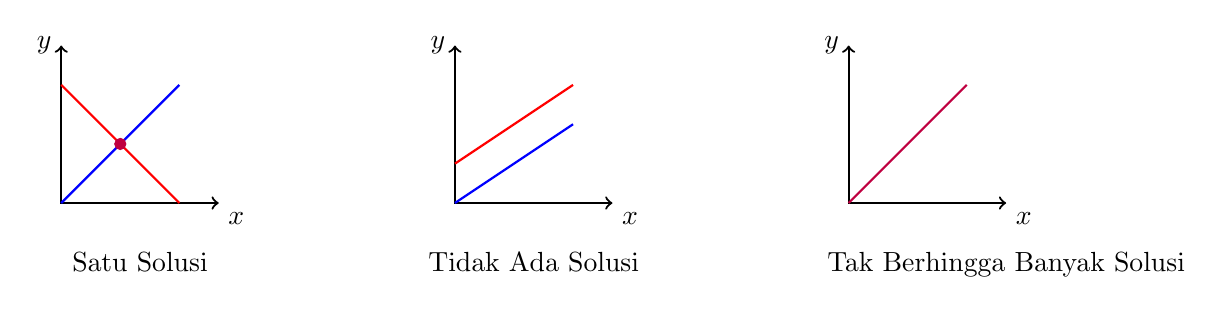
\begin{tikzpicture}
\draw[thick, <->](0,2)--(0,0)--(2,0);
\draw[thick, red](0,1.5)--(1.5,0);
\draw[thick, blue](0,0)--(1.5,1.5);
\draw[fill, purple](0.75,0.75) circle [radius=2pt];
\node[below right] at (2,0){$x$};
\node[left] at (0,2){$y$};
\node[below] at (1,-0.5){Satu Solusi};

\draw[thick, <->](5,2)--(5,0)--(7,0);
\draw[thick, red](5,0.5)--(6.5, 1.5);
\draw[thick, blue](5,0)--(6.5,1);
\node[below right] at (7,0){$x$};
\node[left] at (5,2){$y$};
\node[below] at (6,-0.5){Tidak Ada Solusi};

\draw[thick, <->](10,2)--(10,0)--(12,0);
\draw[thick, purple](10,0)--(11.5, 1.5);
\node[below right] at (12,0){$x$};
\node[left] at (10,2){$y$};
\node[below] at (12,-0.5){Tak Berhingga Banyak Solusi};
\end{tikzpicture}\par\captionof{figure}{Tiga plot 2D berdampingan yang memperlihatkan cara dua garis dapat berpotongan: 'Satu Solusi' (berpotongan di suatu...}\label{fig:systemsofequationsGeometry-tikz01}% fig-num-auto


Pada diagram pertama, terdapat satu titik
perpotongan yang unik, yang berarti bahwa kedua persamaan hanya memiliki satu solusi (unik).
Pada diagram kedua, tidak ada titik perpotongan dan tidak ada solusi. Ketika tidak ada solusi, kedua garis tersebut sejajar dan tidak pernah berpotongan.
Keadaan ketiga yang dapat terjadi, seperti diperlihatkan pada diagram ketiga, adalah bahwa kedua garis itu sebenarnya merupakan garis yang sama. Sebagai
contoh, $x+y=1$ dan $2x+2y=2$ merupakan persamaan yang ketika digambarkan menghasilkan
garis yang sama. Dalam hal ini terdapat tak berhingga banyak titik yang menjadi
solusi kedua persamaan tersebut, karena setiap pasangan terurut yang berada pada grafik
garis itu memenuhi kedua persamaan.
Ketika membahas sistem persamaan linear, selalu terdapat tiga jenis solusi yang mungkin: tepat satu solusi (unik),
tak berhingga banyak solusi, atau tidak ada solusi.

\begin{example}{Solusi Grafis}\label{exa:graphicalsoln}
Gunakan grafik untuk menemukan solusi sistem persamaan berikut \:
\begin{equation*}
\begin{array}{c}
x+y=3 \\
y-x=5
\end{array}
\end{equation*}
\end{example} 

\begin{solution} Dengan menggambarkan persamaan-persamaan di atas dan menentukan titik perpotongannya, kita dapat menemukan solusinya. Ingatlah bahwa hasilnya harus berupa satu solusi, tak berhingga banyak solusi, atau sama sekali tidak ada solusi.
 Grafik berikut memperlihatkan kedua persamaan
beserta perpotongannya. Ingatlah bahwa titik perpotongan merepresentasikan solusi
kedua persamaan, yaitu $\left( x,y\right)$ yang memenuhi keduanya. Dalam hal ini,
terdapat satu titik perpotongan di $\left( -1, 4 \right)$, yang berarti bahwa kita memiliki satu solusi unik, $x = -1, y = 4$.

\begin{center}
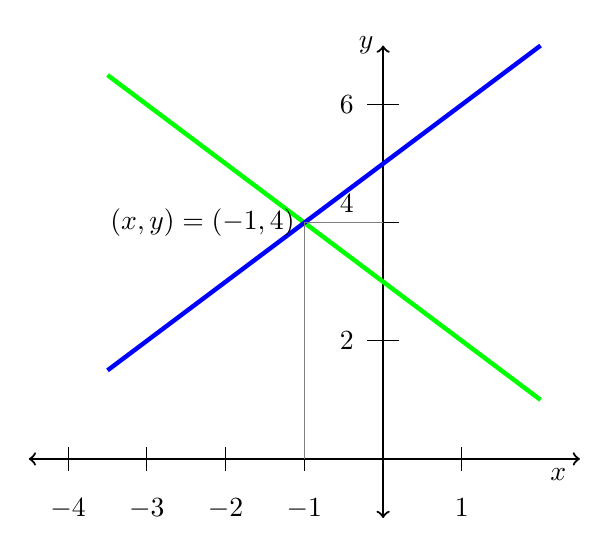
\begin{tikzpicture}[yscale=0.75]
\draw[thick, <->](-4.5,0) -- (2.5,0);
\draw[thick, <->](0,-1) -- (0,7);
\draw(-4,-0.2) -- (-4,0.2);
\draw(-3,-0.2) -- (-3,0.2);
\draw(-2,-0.2) -- (-2,0.2);
\draw(-1,-0.2) -- (-1,0.2);
\draw(1,-0.2) -- (1,0.2);
\draw(-0.2,2) -- (0.2,2);
\draw(-0.2,4) -- (0.2,4);
\draw(-0.2,6) -- (0.2,6);
\draw[green, ultra thick, domain=-3.5:2] plot (\x, {3-\x});
\draw[blue, ultra thick, domain=-3.5:2] plot (\x, {\x+5});
\draw[help lines](-1,0)--(-1,4)--(0,4);
\node[below] at (-4,-0.5){$-4$};
\node[below] at (-3,-0.5){$-3$};
\node[below] at (-2,-0.5){$-2$};
\node[below] at (-1,-0.5){$-1$};
\node[below] at (1,-0.5){$1$};
\node[left] at (-0.25,2){$2$};
\node[above left] at (-0.25,4){$4$};
\node[left] at (-0.25,6){$6$};
\node[below right] at (2,0){$x$};
\node[left] at (0,7){$y$};
\node[left] at (-1,4){$(x,y) = (-1,4)$};
\end{tikzpicture}\par\captionof{figure}{Plot dua dimensi dari sistem x+y=3 dan y-x=5: sebuah garis hijau dan sebuah garis biru yang berpotongan di...}\label{fig:systemsofequationsGeometry-tikz02}% fig-num-auto

\end{center}
\end{solution}

Pada contoh di atas, kita menyelidiki titik perpotongan dua persamaan dalam dua variabel, $x$ dan $y$. Sekarang kita akan membahas
solusi grafis dari tiga persamaan dalam dua variabel.

Perhatikan suatu sistem yang terdiri atas tiga persamaan dalam dua variabel. Sekali lagi, persamaan-persamaan ini dapat digambarkan sebagai
garis lurus pada bidang, sehingga grafik yang dihasilkan memuat tiga garis lurus. Ingat kembali tiga jenis solusi yang mungkin: tidak ada solusi, satu solusi, dan tak berhingga banyak solusi.
Karena kini terdapat garis ketiga, keadaan-keadaan tersebut dapat muncul dengan cara yang lebih rumit. Sebagai contoh, Anda dapat membayangkan tiga garis yang saling berpotongan
tetapi tidak memiliki satu titik perpotongan bersama. Anda mungkin juga dapat membayangkan tiga garis
yang berpotongan pada satu titik. Kedua keadaan ini diperlihatkan di bawah ini.

\begin{center}
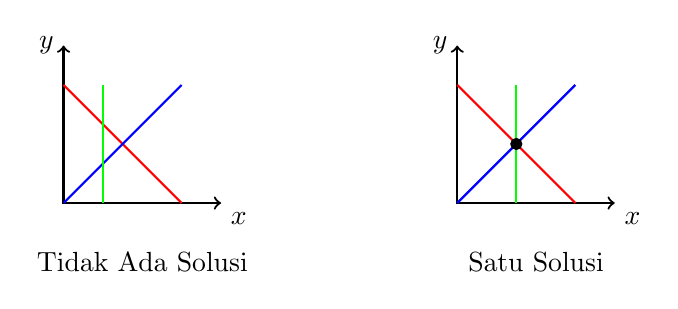
\begin{tikzpicture}
\draw[thick, <->](0,2)--(0,0)--(2,0);
\draw[thick, red](0,1.5)--(1.5,0);
\draw[thick, blue](0,0)--(1.5,1.5);
\draw[thick, green](0.5,0)--(0.5,1.5);
\node[below right] at (2,0){$x$};
\node[left] at (0,2){$y$};
\node[below] at (1,-0.5){Tidak Ada Solusi};

\draw[thick, <->](5,2)--(5,0)--(7,0);
\draw[thick, red](5,1.5)--(6.5,0);
\draw[thick, blue](5,0)--(6.5,1.5);
\draw[thick, green](5.75,0)--(5.75,1.5);
\draw[fill](5.75,0.75) circle [radius=2pt];
\node[below right] at (7,0){$x$};
\node[left] at (5,2){$y$};
\node[below] at (6,-0.5){Satu Solusi};
\end{tikzpicture}\par\captionof{figure}{Dua plot dua dimensi berdampingan yang memperlihatkan tiga garis pada bidang: di sebelah kiri, tiga garis...}\label{fig:systemsofequationsGeometry-tikz03}% fig-num-auto

\end{center}

Perhatikan gambar pertama di atas. Meskipun ketiga garis saling berpotongan, tidak ada satu titik perpotongan bersama
tempat ketiga garis bertemu. Oleh karena itu, ketiga persamaan tersebut tidak memiliki solusi. Ingatlah bahwa solusi adalah titik $\left( x, y \right)$
yang memenuhi \textbf{ketiga} persamaan.
Pada gambar kedua, ketiga garis berpotongan pada satu titik bersama. Artinya, terdapat satu solusi bagi ketiga persamaan yang grafiknya berupa
garis-garis tersebut.
Luangkan waktu sejenak untuk menggambar grafik suatu sistem yang menghasilkan tiga garis sejajar. Selanjutnya, cobalah menggambar grafik tiga garis yang identik. Jenis solusi apa yang direpresentasikan oleh masing-masing grafik tersebut?

Kita telah membahas solusi grafis untuk sistem dua persamaan dalam dua variabel serta tiga persamaan dalam dua variabel. Namun, tidak ada alasan untuk membatasi penyelidikan kita pada persamaan dalam dua variabel. Sekarang kita akan membahas persamaan dalam tiga variabel.

Anda mungkin ingat bahwa persamaan dalam tiga variabel, seperti $2x+4y-5z=8$, membentuk suatu bidang. Di atas, kita mencari perpotongan garis untuk
menentukan solusi yang mungkin. Ketika menyelesaikan sistem persamaan dalam tiga variabel secara grafis, kita mencari
perpotongan bidang. Titik-titik perpotongan ini memberikan $\left( x, y, z \right)$ yang memenuhi semua persamaan
dalam sistem. Jenis solusi apa yang mungkin ketika kita bekerja dengan tiga variabel?
 Perhatikan gambar berikut yang melibatkan dua bidang, yang diberikan oleh dua
persamaan dalam tiga variabel.

\begin{picture}(1,120)
\put(80,30){\begin{picture}(1,1) \thicklines
\setlength{\unitlength}{.3pt} \put(0,0){\line(1,0){300}}
\put(0,0){\line(1,1){75}}\put(300,150){\line(1,0){150}}\put(450,150){\line(-1,-1){150}
}\put(150,0){\line(1,1){150}}\put(150,0){\line(-1,1){100}}\put(50,100){\line(1,1){150}}
\put(200,250){\line(1,-1){100}}\put(75,75){\qbezier[14](0,0)(37.5,37.5)(75,75)}
\put(150,150){\qbezier[14](0,0)(75,0)(150,0)}\put(300,150){\qbezier[14](0,0)(37.5,-37.5)(75,-75)}
\put(375,75){\line(1,-1){20}}\put(395,55){\line(-1,-1){150}}
\put(150,0){\line(1,-1){95}}
\end{picture}}
\end{picture}\par\captionof{figure}{Dua bidang yang berpotongan pada sebuah garis.}\label{fig:planes-intersect-line}% fig-num-auto


Perhatikan bahwa kedua bidang ini berpotongan pada sebuah garis. Artinya, titik-titik $\left( x,y,z\right)$ pada garis ini
memenuhi kedua persamaan dalam sistem. Karena garis tersebut memuat tak berhingga banyak titik, sistem ini memiliki tak berhingga banyak solusi.

Kedua bidang juga mungkin tidak berpotongan. Namun, mungkinkah dua bidang berpotongan hanya pada satu titik? Luangkan waktu sejenak untuk mencoba menggambar keadaan tersebut dan yakinkan diri Anda bahwa hal itu
tidak mungkin! Artinya, jika kita hanya memiliki dua persamaan dalam tiga variabel, solusi unik tidak mungkin ada. Jadi, jenis solusi yang mungkin bagi dua persamaan dalam tiga variabel adalah tidak ada solusi atau tak berhingga banyak solusi.

Sekarang bayangkan kita menambahkan bidang ketiga. Dengan kata lain, perhatikan tiga persamaan dalam tiga variabel. Jenis solusi apa yang kini mungkin? Perhatikan diagram berikut.

\begin{picture}(1,120)
\put(80,30){\begin{picture}(1,1) \thicklines
\setlength{\unitlength}{.3pt} \put(0,0){\line(1,0){300}}
\put(0,0){\line(1,1){50}}\put(300,150){\line(1,0){150}}\put(450,150){\line(-1,-1){150}
}\put(150,0){\line(1,1){150}}\put(150,0){\line(-1,1){100}}\put(50,100){\line(1,1){150}}
\put(200,250){\line(1,-1){50}}
\put(250,200){\qbezier[3](0,0)(12.5,-12.5)(25,-25)}
\put(275,175){\line(1,-1){25}}
\put(50,50){\qbezier[18](0,0)(50,50)(100,100)}
\put(150,150){\qbezier[14](0,0)(75,0)(150,0)}\put(300,150){\qbezier[14](0,0)(37.5,-37.5)(75,-75)}
\put(375,75){\line(1,-1){20}}\put(395,55){\line(-1,-1){150}}
\put(150,0){\line(1,-1){95}}\put(100,50){\line(1,1){150}}\put(100,50){\line(-1,0){120}}
\put(-20,50){\line(1,1){150}}\put(130,200){\line(1,0){20}}
\put(140,200){\qbezier[10](0,0)(50,0)(110,0)}\put(250,200){\line(1,0){50}}
\put(300,200){\line(-1,-1){150}} \put(150,50){\line(-1,0){50}}
\put(320,230){\vector(-1,-1){30}}\put(325,230){New Plane}
\end{picture}}
\end{picture}\par\captionof{figure}{Tiga bidang tanpa titik perpotongan bersama.}\label{fig:planes-no-common-point}% fig-num-auto


Pada diagram ini, tidak ada titik yang terletak pada ketiga bidang. Tidak ada perpotongan di antara \textbf{semua} bidang,
sehingga tidak ada solusi. Gambar tersebut
memperlihatkan keadaan ketika garis perpotongan bidang baru
dengan salah satu bidang semula membentuk garis yang sejajar dengan garis
perpotongan kedua bidang pertama. Namun, dalam tiga dimensi,
dua garis mungkin tidak berpotongan meskipun keduanya tidak
sejajar. Garis semacam itu disebut \textbf{garis bersilangan}.
\index{garis bersilangan}

Ingatlah bahwa ketika bekerja dengan dua persamaan dalam tiga variabel, solusi unik tidak mungkin ada. Apakah solusi unik mungkin
ketika kita membahas tiga persamaan dalam tiga variabel? Ternyata mungkin, dan keadaan tersebut diperlihatkan pada gambar berikut.

\begin{picture}(1,120)
\put(90,30){\begin{picture}(1,1) \thicklines
\setlength{\unitlength}{.3pt} \put(0,0){\line(1,0){300}}
\put(0,0){\line(1,1){75}}
\put(300,150){\line(1,0){150}}
\put(300,150){\qbezier[4](0,0)(25,0)(50,0)}
\put(350,150){\line(1,0){100}}
 \put(450,150){\line(-1,-1){150}}
\put(150,0){\line(1,1){50}}
\put(200,50){\qbezier[14](0,0)(50,50)(100,100)}
\put(150,0){\line(-1,1){100}}\put(50,100){\line(1,1){150}}
\put(200,250){\line(1,-1){100}}
\put(200,250){\qbezier[14](0,0)(50,-50)(100,-100)}
\put(75,75){\qbezier[14](0,0)(37.5,37.5)(75,75)}
\put(150,150){\qbezier[14](0,0)(75,0)(150,0)}\put(300,150){\qbezier[14](0,0)(37.5,-37.5)(75,-75)}
\put(375,75){\line(1,-1){20}}
 \put(395,55){\line(-1,-1){45}}
 \put(350,10){\qbezier[6](0,0)(-27,-27)(-60,-60)}
 \put(290,-50){\line(-1,-1){45}}
\put(150,0){\line(1,-1){95}}\put(200,50){\line(0,1){200}}\put(200,50){\line(1,0){150}}
\put(200,50){\qbezier[10](0,0)(-50,0)(-100,0)}\put(100,50){\line(-1,0){50}}
\put(50,50){\line(0,1){200}} \put(350,50){\line(0,1){200}}
\put(350,250){\line(-1,0){300}} \put(200,50){\circle*{5}}
\put(350,50){\line(0,-1){100}}\put(200,50){\qbezier[4](0,0)(0,-25)(0,-50)}
\put(200,0){\line(0,-1){50}} \put(200,-50){\line(1,0){150}}
\put(200,-50){\line(-1,0){150}} \put(50,-50){\line(0,1){50}}
\put(50,0){\qbezier[4](0,0)(0,25)(0,50)}
\put(400,250){\vector(-1,-1){50}} \put(405,250){New Plane}
\end{picture}}
\end{picture}\par\captionof{figure}{Tiga bidang yang berpotongan pada satu titik.}\label{fig:planes-single-point}% fig-num-auto


Dalam hal ini, ketiga bidang memiliki satu titik perpotongan.
Dapatkah Anda memikirkan jenis solusi lain yang mungkin? Kemungkinan lainnya adalah
ketiga bidang berpotongan pada sebuah garis, sehingga menghasilkan tak berhingga banyak solusi, seperti pada diagram berikut.

\begin{picture}(1,120)
\put(80,30){\begin{picture}(1,1) \thicklines
\setlength{\unitlength}{.3pt} \put(0,0){\line(1,0){300}}
\put(0,0){\line(1,1){75}}
 \put(300,150){\line(1,0){150}}
 \put(450,150){\line(-1,0){83.333}}
 \put(300,150){\qbezier[6](0,0)(33,0)(66,0)}
\put(450,150){\line(-1,-1){150}
}\put(150,0){\line(1,1){150}}\put(150,0){\line(-1,1){100}}\put(50,100){\line(1,1){150}}
\put(200,250){\line(1,-1){100}}\put(75,75){\qbezier[14](0,0)(37.5,37.5)(75,75)}
\put(150,150){\qbezier[14](0,0)(75,0)(150,0)}\put(300,150){\qbezier[14](0,0)(37.5,-37.5)(75,-75)}
\put(375,75){\line(1,-1){20}}\put(395,55){\line(-1,-1){150}}
\put(150,0){\line(1,-1){95}}\put(150,0){\line(-3,-1){90}}
\put(60,-30){\line(1,1){30}}
\put(150,0){\line(3,1){100}}\put(250,33.333){\line(1,1){150}}
\put(400,183.333){\line(-3,-1){100}}
\end{picture}}
\end{picture}\par\captionof{figure}{Bidang ketiga yang melalui garis perpotongan dua bidang.}\label{fig:planes-new-plane}% fig-num-auto


Kita telah melihat bahwa tiga persamaan dalam tiga variabel dapat tidak memiliki solusi, memiliki solusi unik, atau berpotongan pada suatu garis sehingga menghasilkan tak berhingga banyak solusi.
Ketiga persamaan juga mungkin menggambarkan bidang yang sama, yang juga menghasilkan tak berhingga banyak solusi.

Anda dapat melihat bahwa ketika bekerja dengan persamaan dalam tiga variabel, terdapat
jauh lebih banyak cara untuk menghasilkan berbagai jenis solusi daripada ketika bekerja dengan dua variabel. Akan bermanfaat jika Anda
meluangkan waktu untuk membayangkan (dan menggambar) berbagai keadaan yang mungkin; cobalah beberapa di antaranya.

Anda juga sebaiknya meluangkan waktu untuk membayangkan (dan menggambar) grafik sistem dengan lebih dari tiga variabel.
Persamaan seperti $x+y-2z+4w=8$ yang memiliki lebih dari tiga variabel sering disebut \textbf{hiperbidang}. \index{hiperbidang}
Anda akan segera menyadari bahwa grafik hiperbidang sulit digambar. Dengan alat-alat aljabar linear,
kita dapat mengkaji secara aljabar jenis-jenis sistem yang sulit digambarkan ini. Pada bagian berikutnya, kita akan membahas alat-alat
aljabar tersebut.
